%%  Language: 
%%      finnish, swedish, or english
%%  Pagination (use twoside by default)  
%%      oneside or twoside,
%%  Study programme / kind of report
%%      csm  = Master's thesis in Computer Science Master's Programme;
%%      tkt = Bachelor's thesis in Computer Science Bachelor's Programme;
%%      seminar = seminar report
%%  For Master's thesis choose your line or track:
%%      (30 cr thesis, 2020 onwards, Master's Programme in Computer Science = csm)
%%      software-track-2020 = Software study track
%%      algorithms-track-2020 = Algorithms study track
%%      networking-track-2020 = Networking study track

\documentclass[finnish,twoside,censored,tkt]{HYthesisML} 


% If wanted, open new chapters only at right page.
% By default, "openany".
%\PassOptionsToClass{openright,twoside,a4paper}{report}
\PassOptionsToClass{openany,twoside,a4paper}{report}

\usepackage{csquotes}
%%%%%%%%%%%%%%%%%%%%%%%%%%%%%%%%%%%%%%%%%%%%%%%%%%%%%%%%%
%% REFERENCES
%% Some notes on bibliography usage and options:
%% natbib -> you can use, e.g., \citep{} or \parencite{} for (Einstein, 1905); with APA \cite -> Einstein, 1905 without ()
%% maxcitenames=2 -> only 2 author names in text citations, if more -> et al. is used
%% maxbibnames=99 as no great need to suppress the biliography list in a thesis
%% for more information see biblatex package documentation, e.g., from https://ctan.org/pkg/biblatex 

%% Reference style: select one 
%% for APA = Harvard style = authoryear -> (Einstein, 1905) use:
\usepackage[style=authoryear,bibstyle=authoryear,backend=biber,natbib=true,maxnames=99,maxcitenames=99,uniquelist=minyear,giveninits=true,uniquename=mininit]{biblatex}
%% for numeric = Vancouver style -> [1] use:
%\usepackage[style=numeric,bibstyle=numeric,backend=biber,natbib=true,maxbibnames=99,giveninits=true,uniquename=init]{biblatex}
%% for alpahbetic -> [Ein05] use:
%\usepackage[style=alphabetic,bibstyle=alphabetic,backend=biber,natbib=true,maxbibnames=99,giveninits=true,uniquename=init]{biblatex}
%

\addbibresource{bibliography.bib}
% in case you want the final delimiter between authors & -> (Einstein & Zweistein, 1905) 
% \renewcommand{\finalnamedelim}{ \& }
% List the authors in the Bibilipgraphy as Lastname F, Familyname G,
\DeclareNameAlias{sortname}{family-given}
% remove the punctuation between author names in Bibliography 
%\renewcommand{\revsdnamepunct}{ }


%% Block of definitions for fonts and packages for picture management.
%% In some systems, the figure packages may not be happy together.
%% Choose the ones you need.

\usepackage[utf8]{inputenc} % For UTF8 support, in some systems. Use UTF8 when saving your file.

\usepackage{lmodern}         % Font package, again in some systems.
\usepackage{textcomp}        % Package for special symbols
\usepackage[pdftex]{color, graphicx} % For pdf output and jpg/png graphics
\usepackage{epsfig}
\usepackage{subfigure}
\usepackage[pdftex, plainpages=false]{hyperref} % For hyperlinks and pdf metadata
\usepackage{fancyhdr}        % For nicer page headers
\usepackage{tikz}            % For making vector graphics (hard to learn but powerful)
%\usepackage{wrapfig}        % For nice text-wrapping figures (use at own discretion)
\usepackage{amsmath, amssymb} % For better math
\usepackage{microtype} % For better math

\singlespacing               %line spacing options; normally use single

\fussy
%\sloppy                      % sloppy and fussy commands can be used to avoid overlong text lines
% if you want to see which lines are too long or have too little stuff, comment out the following lines
% \overfullrule=1mm
% to see more info in the detailed log about under/overfull boxes...
% \showboxbreadth=50 
% \showboxdepth=50



%%%%%%%%%%%%%%%%%%%%%%%%%%%%%%%%%%%%%%%%%%%%%%%%%%%%%%%%%
%% STEP 2:
%%%%%%%%%%%%%%%%%%%%%%%%%%%%%%%%%%%%%%%%%%%%%%%%%%%%%%%%%
%% Set up personal information for the title page and the abstract form.
%% Replace parameters with your information.
\title{Paikallisherkkien tiivistefunktioiden soveltaminen haittaohjelmien tunnistamisessa}

\author{Nuutti Varvikko}
\date{\today}

% Set supervisors, use the titles according to the thesis language
% in English Prof. or Dr., or in Finnish toht. or tri or FT, TkT, Ph.D. or in Swedish... 
\supervisors{prof. Nikolaj Tatti}

\keywords{similarity hashing, fuzzy hashing, malware detection}
\additionalinformation{\translate{\track}}

%% For seminar reports:
%%\additionalinformation{Name of the seminar}

%% Provide classification terms, to appear on the abstract page.
%% Replace the classification terms below with the ones that match your work.
%% ACM Digital library provides a taxonomy and a tool for classification
%% in computer science. Use 1-3 paths, and use right arrows between the
%% about three levels in the path; each path requires a new line.

% \classification{\protect{\ \\
% \  General and reference $\rightarrow$ Document types  $\rightarrow$ Surveys and overviews\  \\
% \  Applied computing  $\rightarrow$ Document management and text processing  $\rightarrow$ Document management $\rightarrow$ Text editing
% }}

\classification{\protect{\ \\
\  Security and privacy $\rightarrow$ Cryptography $\rightarrow$ Symmetric cryptography and hash functions $\rightarrow$ Hash functions and message authentication codes\ \\
\  Security and privacy $\rightarrow$ Intrusion/anomaly detection and malware mitigation $\rightarrow$ Malware and its mitigation
}}
%% If you want to quote someone special. You can comment this line out and there will be nothing on the document.
%\quoting{Bachelor's degrees make pretty good placemats if you get them laminated.}{Jeph Jacques}


%% OPTIONAL STEP: Set up properties and metadata for the pdf file that pdfLaTeX makes.
%% Your name, work title, and keywords are recommended.
\hypersetup{
    unicode=true,           % to show non-Latin characters in Acrobat’s bookmarks
    pdftoolbar=true,        % show Acrobat’s toolbar?
    pdfmenubar=true,        % show Acrobat’s menu?
    pdffitwindow=false,     % window fit to page when opened
    pdfstartview={FitH},    % fits the width of the page to the window
    pdftitle={},            % title
    pdfauthor={},           % author
    pdfsubject={},          % subject of the document
    pdfcreator={},          % creator of the document
    pdfproducer={pdfLaTeX}, % producer of the document
    pdfkeywords={something} {something else}, % list of keywords for
    pdfnewwindow=true,      % links in new window
    colorlinks=true,        % false: boxed links; true: colored links
    linkcolor=black,        % color of internal links
    citecolor=black,        % color of links to bibliography
    filecolor=magenta,      % color of file links
    urlcolor=cyan           % color of external links
}

%%-----------------------------------------------------------------------------------

\begin{document}

% Generate title page.
\maketitle

% \begin{abstract}{finnish}

% Tämä dokumentti on tarkoitettu Helsingin yliopiston tietojenkäsittelytieteen osaston opin\-näyt\-teiden ja harjoitustöiden ulkoasun ohjeeksi ja mallipohjaksi. Ohje soveltuu kanditutkielmiin, ohjelmistotuotantoprojekteihin, seminaareihin ja maisterintutkielmiin. Tämän ohjeen lisäksi on seurattava niitä ohjeita, jotka opastavat valitsemaan kuhunkin osioon tieteellisesti kiinnostavaa, syvällisesti pohdittua sisältöä.


% Työn aihe luokitellaan  
% ACM Computing Classification System (CCS) mukaisesti, 
% ks.\ \url{https://dl.acm.org/ccs}. 
% Käytä muutamaa termipolkua (1--3), jotka alkavat juuritermistä ja joissa polun tarkentuvat luokat erotetaan toisistaan oikealle osoittavalla nuolella.

% \end{abstract}

\begin{otherlanguage}{english}
\begin{abstract}

Tiivistys on yleisesti käytetty menetelmä haittaohjelmien tunnistamiseen.
Erityisesti moderneista haittaohjelmmista levitetään tyypillisesti
muunneltuja versioita, joita on vaikeampi tunnistaa. Kryptografisilla
tiivisteillä ei voida tunnistaa tällaisia samankaltaisia ohjelmia.
Samankaltaisuuksinen tunnistamiseen on kehitetty erilaisia sumeita tiivisteitä,
jotka kykenevät yhdistämään suurestikin poikkeavia syötteitä toisiinsa.
Sumeita tiivistetiä on paljon, ja paikoitellen ne eroavat toisistaan
merkittävästi. Tässä tutkielmassa käsitellään sumeiden tiivisteiden
soveltamista haittaohjelmien tunnistamiseen niiden
sisältämien samankaltaisuuksien perusteella. Erityisesti analysoidaan
eri ohjelmistojen soveltuvuutta ja puutteita sekä sumean tiivistyksen
haavoittuvuuksia.

\end{abstract}
\end{otherlanguage}


% Place ToC
%\newpage
\mytableofcontents

\mainmatter

\chapter{Johdanto\label{intro}}
 
Tietojenkäsittelyssä käsitellään valtavia määriä dataa. Laskentakyvyn kasvessa myös tiedonsiirto-
ja tallenuskapasiteetti kehittyvät, ja tietojenkäsittelyn kehitys luo myös rikollisia intressejä
edistäviä mahdollisuuksia. Sekä tekninen rikostutkinta että kyberrikollisuus ovat riippuvaisia
tietotekniikan kehityksestä. Uudet innovaatiot synnyttyävät mahdollisuuksia kehittää rikollisia
menetelmiä sekä toisaalta ratkaisuja haitallista toimintaa vastaaan.

Kasvava datavirta helpottaa haittaohjelmien huomaaamatonta leviämistä, ja haittaohjelma saattaa
jäädä kokonaan huomaamatta. Haittaohjelmien torjuntaa voidaan tietoisesti pyrkiä johtamaan harhaan
aiheuttamalla aiheettomia osumia. Haitallisen datan tunnistaminen kasvavasta tietoliikenteestä
edellyttää kohdennettuja resursseja sekä suorituskykyisiä ratkaisuja. Tiedon esittämiselle
kompaktimmassa muodossa onkin tarvetta sen tehokkaan tunnistamisen vuoksi.

Dataa voidaan tiivistää muun muassa pakkaus- ja tiivisteohjelmistoilla. Pakkauksesta poiketen
tyypillisesti käytetyt kryptografiset tiivistefunktiot tiivistävät datan palauttamattomaan muotoon.
Toisaalta tiiviste sisältää lähes uniikin tunnisteen, jolla alkuperäinen data on käytännössä
tunnistettavissa. Tiivistystä voidaankin hyödyntää menetelmänä haittaohjelmien havaitsemisessa
suuresta datamäärästä. Tyypillisesti tunnistetuista haittaohjelmista on luotu tiiviste, jolloin
saman tiivisteeen tuottavaa ohjelmaa voidaan epäillä haittaohjelmaksi. Mikä tahansa muutos tuottaa
kuitenkin tunnistamattomaan tiiviisteen perinteisesti tarkoitukseen käytetyillä kryptografisilla
tiivistefunktioilla. Rikolliset tahot pyrkivät kiertämään haittaohjelmien torjuntamenetelmiä
esimerkiksi tekemällä ohjelmistoon muutoksia. Muutettua haittaohjelmaa ei voida enää tunnistaa
alkuperäiseksi tiivisteitä vertaamalla, vaikka toiminnallisuudeltaan ohjelma olisi identtinen.

Seuraavassa luvussa esitellään yleisesti sumean tiivisteen käsite sekä taustoitetaan eri
tiivistetyyppien toimintaperiaate. Luvussa 3 käydään läpi kolme sumeiden tiivisteiden
prosessointiin käytettyä ohjelmistoa: Ssdeep, Sdhash sekä Mvhash-b. Luvussa 4 käsitellään
sumeiden tiivsteiden soveltamista haittaohjelma-analyysissa edellytyksineen. Lisäksi luvussa
analysoidaan menetelmiä, joilla haittaohjelmien tunnistamista sumein tiivistein voidaan johtaa
harhaan. Luvussa 5 käsitellään sumean tiivistämisen heikkouksia sekä tarkastellaan ohjelmistojen
eroavaisuuksien merkitystä haittaohjelma-analyysissa.

\chapter{Sumea tiiviste\label{fuzzy-hash}}

% 4

Kryptografisia tiivisteitä käytetään laajasti datan tunnistamiseen \parencite{kornblum06}. Ne tuottavat
samalla syötteellä saman tiivisteen, ja data voidaan lähes varmuudella tunnistaa
samaksi yhtäläisen tiivisteen perusteella. Pieninkin muutos syötteessä tuottaa
kuitenkin aiemmasta tunnistamattoman tiivisteen. Vertailu kryptografisilla
tiivisteillä ei ole soveltuva keino samankaltaisten syötteiden tunnistamiseen
\citep{kornblum06}.

Samankaltaisuuden tunnistamista varten kehitetyillä sumeilla tiivisteillä
voidaan vaivatta tunnistaa toisistaan eroavia samankaltaisia syötteitä \parencite{kornblum06}. Sumeat
tiivisteet mahdollistavat suurestikin muutettujen tai puutteellisten tiedostojen
yhdistämisen alkuperäiseen versioon. Samanakaltaisuuksien tunnistamisella
on merkitystä myös haittaohjelma-analyysissa. Haittaohjelmia
kehittävillä tahoilla on taipumus toistaa kaavamaisia piirteitä,
joten yhden tunnistetun haittaohjelman avulla voidaan mahdollisesti
havaita muitakin haittaohjelmia \parencite{naik19}.

Tässä tutkielmassa sumeat tiivisteet jaetaan toimintaperiaatteen
mukaan luokkiin perustuen luokitukseen, jonka \textcite{martin-perez21}
esittelevät.
Tiivisteet on jaettu ominaisuuksiensa perusteella kolmeen luokkaan.
Seuraavassa aliluvussa käsitellään sumeiden tiivistefunktioiden
toimintaa yleisellä tasolla. Viimeisissä aliluvuissa käsitellään
kaksi sumeiden tiivisteiden luokkaa: tiivistetyt ominaisuusjonot sekä
tavujonot.

\section{Tiivistäminen ja vertailu}

Samankaltaisuuksia tunnistavia algoritmeja laatiessa keskitytään
koko syötteen tarkastelun sijaan pieniin osioihin.
Olennaista ei ole tunnistaa täsmälleen tietynlaista syötettä,
vaan löytää syötteestä vertailuun sopivia säännönmukaisuuksia. Näitä
rakenteita kutstuaan usein ominaisuuksiksi \parencite{martin-perez21}.
Ominaisuuksien valintakriteerit ja vertauslogiikka riippuvat
käytetystä algoritmista.

Monet algoritmit muodostavat sumean tiivisteen jonosta, joka
sisältää syötteestä valitut ominaisuudet tiivistettynä \parencite{martin-perez21}.
Osa tiivisteistä tiivistää koko syötteen, toisaalta
osa tiivistää ainoastaan osan. Huomionarvoista
on, että ominaisuuksien tiivistämiseen käytetään
sumeisssakin tiivisteissä kryptografisia tiivisteitä \parencite{kornblum06}.
Datan samankaltaisuuden vertailu sumeilla tiivisteillä etenee
vertaillen tiivistettyjä ominaisuuksia koko tiivisteen sijaan.
Samankaltaisuuden mittarina käytettävä ominaisuuksien
vertailufunktio riippuu käytetystä algoritmista.

\section{Tiivistetyt ominaisuusjonot}

Ominaisuusjonojen tiivistäminen on sumeiden tiivisteiden luokka,
johon kuuluu useita laajalti käytettyjä tiivisteitä. \textcite{martin-perez21}
esittävät tiivistetyt ominaisuusjonot yhtenä kolmesta tiivisteluokasta.
Tässä lähestymistavassa tarkastellaan ominaisuuksista
muodostuvia jonoja, eli syötteestä etsitään ominaisuuksia,
jotka tiivistetään jonoksi. Piirteen määrittely sekä
valinta on algoritmikohtaista.

\begin{table}[h]
   \centering
   \caption{Merkkijonolle luotu tiiviste, joka on määritelty paloittain.}
   \begin{tabular}{|c|c|c|c|c|c|c|c|c|c|c|c|} 
      \hline
      h & e & i                  &  & m & a                & a & i & l               & m & a & !                \\ 
      \hline
      \multicolumn{3}{|c|}{7b}   & \multicolumn{3}{c|}{7f} & \multicolumn{3}{c|}{e5} & \multicolumn{3}{c|}{53}  \\
      \hline
   \end{tabular}
\end{table}

Tiivistetty ominaisuusjono voidaan muodostaa määrittelemällä
tiiviste paloittain \parencite{martin-perez21}. Syöte jaetaan lohkoihin,
jolloin suuresta syötteestä muodostuu jono vertailtavia ominaisuuksia. 
Yksinkertaisessa paloittaisessa määrittelyssä syöte jaetaan
vakiokokoisiin lohkoihin, jotka kuvaavat syötteen ominaisuuksia
\parencite{kornblum06}.
Paloittain määritelty tiiviste muodostuu siis jonosta tiivistettyjä
lohkoja $H_i = R(a_j, a_{j - 1}, a_{j - 2}, \dots, a_{j - n})$,
missä $n$ käytetty lohkokoko ja $j = in$. Menetelmää havainnollistetaan
taulukossa 2.1, jossa syötteen lohkoille generoidaan tiivisteet
CRC-8-tiivistefunktiolla lohkokoon ollessa $n = 3$.

\begin{table}[h]
   \centering
   \caption{Paloittain määritelty tiiviste merkkijonolle, jossa merkkejä
      on vaihdettu.}
   \begin{tabular}{|c|c|c|c|c|c|c|c|c|c|c|c|} 
      \hline
      \textcolor{red}{h} & e & i                  &  & m & a                & a & i & l               & m & a & \textcolor{red}{?}                \\ 
      \hline
      \multicolumn{3}{|c|}{\textcolor{red}{38}}   & \multicolumn{3}{c|}{7f} & \multicolumn{3}{c|}{e5} & \multicolumn{3}{c|}{\textcolor{red}{09}}  \\
      \hline
   \end{tabular}
\end{table}

Taulukossa 2.2 on kuvattu muutoksia, jotka aiheutuvat, kun syötteen
alkioita vaihdetaan. Koska syötteen pituus säilyy muuttumattomana, muutokset
heijastuvat ainoastaan lohkoihin, joissa muutoksia on tapahtunut; keskimmäisten
lohkojen tiivisteet eivät ole muuttuneet lainkaan. Sen sijaan taulukossa 2.3
huomataan algoritmin toiminnan häiriintyvän pahasti, kun syötteen pituus muuttuu.
Alkion lisäys tai poisto muuttaa kyseistä alkiota seuraavien alkoiden indeksiä.
Syötteen alkuun lisätty alkio johtaa pahimmillaan kaikkien seuraavien lohkojen
tiivisteen muuttumisen tunnistamattomaksi.

\begin{table}[h]
   \centering
   \caption{Paloittain määritelty tiiviste johon on lisätty merkki.}
   \begin{tabular}{|c|c|c|c|c|c|c|c|c|c|c|c|c|} 
      \hline
      H & e & i                  & \textcolor{red}{,} &  & m                & a & a & i                                & l & m & a                                & !                    \\ 
      \hline
      \multicolumn{3}{|c|}{7b}   & \multicolumn{3}{c|}{\textcolor{red}{e9}} & \multicolumn{3}{c|}{\textcolor{red}{54}} & \multicolumn{3}{c|}{\textcolor{red}{03}} & \textcolor{red}{e7}  \\
      \hline
   \end{tabular}
\end{table}

Vakiokokoisilla lohkoilla esiintyvä ongelma ratkeaa, kun lohko sisältää saman
alkiojonon lisäyksistä riippumatta \parencite{kornblum06}. Kontekstiriippuvaisessa paloittaisessa tiivistyksessä
lohkot määritetään syötteen perusteella. Algoritmin toimintaperiaatteena on jakaa syöte
lohkoiksi siten, että lohkot sisältävät algoritmille määritellyn kontekstin.
Kontekstiriippuva paloittain määritelty tiiviste ei ole herkkä syötteen pituuden
muuttumisel le. Lisäämistä ja poistamisesta vaikuttaa ihanteellisesti yhden,
ja enimmilläänkin vain lähimpien naapurilohkojen tiivisteisiin eikä heijastu muihin lohkoihin.

Paloittaisen määritettelyn lisäksi sumeaa tiivistystä on lähestytty muilla tavoilla.
lohkoihin jakamisen sijaan syötteeestä voidaan etsiä tilastollisesti poikkeavia
piirteitä. Poikkeavia piirteitä havainnoiva algoritmi valitsee tietyn määrän
poikkeavimpia piirteitä ja tiivistää ne \citep{roussev10}. Varsinainen sumea tiiviste muodostuu
valittujen piirteiden tiivisteistä. Paloittain määriteltyjen tiivisteiden tavoin
tiivistämiseen käytetään kryptografista tiivistefunktiota. Huomionarvoista on,
että yleensä tiivistettäväksi valitut ominaisuudet kattavat syötteestä ainoastaan osan \citep{martin-perez21}.
Syötteestä ei siis tiivistetä kuin osa, toisin kuin paloittain määritteltäessä.

Poikkeavuudet säilyttävän tiivisteen lähestymistavassa tulkitaan,
että samalla tavalla merkittävästi poikkeavat syötteet liittyvät
toisiinsa. Ei siis ole todennäköistä, että satunnaisissa syötteissä
esiintyisi suuri määrä samoja, epätyypillisiä piirteitä. Kuvatussa
tilanteessa on pääteltävissä syötteiden olevan mitä luultavimmin
peräisin samasta alkuperästä, ja piirteet ovat muokkausten jälkeen
jääneet yhdistäväksi tekijäksi. Tällöin voidaan tehdä johtopäätös
ja olettaa syötteiden olevan tietyllä todennäköisyydellä
kokonaisuutenakin samankaltaisia.

Poikkeavuuksiin perustuvuvan algoritmin on etsittävä
syötteestä piirteet ja valittava niistä epätyypillisimmät.
Keskeinen ongelma onkin piirteen määrittely. Onglemaan
ei ole yksikäsitteistä ratkaisua, ja määritelmä
on tapauskohtaista. Esimerkiksi seuraavassa luvussa
käsiteltävässä Sdhash-ohjelmistossa piirre on määritelty
64 tavun merkkijonoksi \citep{roussev10}.
% ^ cyber threat hunting
% Breitinger et al.(Breitinger & Baier, 2012b)showed some weaknesses in sdhash and pre-sented improvements to the scheme | security analysis
% However, its strong suit is the detection of fragments and not comparison of files [p.8, breitinger12].


\section{Tavujono}

Tavujonosyötteet muodostavat tiivisteen jakamalla syötteen lohkoiksi,
joita verrataan samankaltaisuuden perusteella yhtäsuuruuden sijaan
\parencite{martin-perez21}.
Lohkoista rakennetaan syötteelle uusi esitystapa, joka sisältää
yksinkertaistetun kuvauksen syötteestä. Muutokset alkuperäisessä
syötteessä eivät vaikuta tietyissä rajoissa yksinkertaistettuun
muotoon, jonka perusteella samankaltaisuudet voidaan edelleen
määrittää. Tavujonotiivisteet eivät etsi syötteestä tietyntyyppisiä
ominaisuuksia kuten ominaisuustiivisteet.

Tavujonotiivisteille on määriteltävä logiikka, jolla lohkonta
suoritetaan. Lohkot voivat olla myös vakiokokoisia, jos niiden
tiivistykseen ei käytetä kryptografista tiivistettä; esimerkiksi
Mvhash-b-ohjelmistossa lohkot ovat vakiokokoisia. Lohkon arvoksi
asetetaan joko 0 tai 255, riippuen alkioiden enemmistöstä.
Enemmistöperiaatteen sekä arvojen pienen määrän vuoksi lohkosta
toiseen siirtyvien alkioiden vaikutus häipyy.


\chapter{Sumean tiivistämisen ohjelmistot\label{fuzzy-software}}

% 5

\section{Ssdeep}

Ssdeep on laajasti käytetty ohjelmisto kontekstiriippuvaisten paloittain
määriteltyjen tiivisteiden prosessointiin \citep{gayoso15}. Syötteiden
vertailu paloittain määritellyin tiivistein tapahtuu kahdessa vaiheessa.
Tiivisteet on ensin generoitava, minkä jälkeen samankaltaisuuden vertaaminen
tapahtuu tiivisteitä verraten. Ssdeepillä voidaan generoida kontekstitiippuvainen tiiviste tidostoille ja vertailla generoituja tiivisteitä keskenään.

Taulukko 3.1 havainnollistaa ssdeep-ohjelmiston käyttöä. Kahdelle
JavaScript-lähdekooditie\-dostolle generoidaan tiivisteet. Tämän
jälkeen saatuja tiivisteitä verrataan Ssdeepin vertailutilassa, joka
ilmaisee, ovatko syötteet samankaltaisia. Ssdeep määrittää samankaltaisuuden
suljetulla välillä $[0, 100]$, missä 0 tarkoittaa pienintä havaittavaa
vastaavuutta, ja 100 täydellistä vastaavuutta \citep{kornblum06}.
Mikäli Ssdeep ei kykene tulkitsemaan syötteitä samankaltaisiksi,
komento ei tulosta mitään.

\begin{table}[h]
  \caption{Alkuperäisen ja muokatun lähdekooditiedoston luonti ja vertailu ssdeep-ohjelmistolla.}
  \begin{verbatim}
   $ ssdeep -l functional.js functional-uncommented.js
  ssdeep,1.1--blocksize:hash:hash,filename
  192:eQiHcd9A+QKxYI1LIgbKvgiuqB0ML2lJGnYDTo/Z:Acd9A+QKlLpbKJ01lJQYDGZ,
    "functional.js"
  192:oQ+BA+QKNYI1LIPuiuqW0ML2lJGnYDTo/Z:KA+QKJLp01lJQYDGZ,
    "functional-uncommented.js"

  $ ssdeep -lrd functional.js functional-uncommented.js
  functional-uncommented.js matches functional.js (75)
  \end{verbatim}
\end{table}

Ssdeepin generoima tiiviste muodostuu varsinaisen tiivisteen lisäksi
lohkokoon osoittavasta kokonaisluvusta sekä syötetyn tiedoston polusta.
Lohkokoko riippuu syötteenä
annetun datan pituudesta \citep{kornblum06}. Itse tiiviste muodostuu kahdesta kaksoispisteellä erotetusta tiivisteestä.
Ssdeep iteroi syötteen uudelleen käyttäen laukaisimena kaksinkertaista
lohkokokoa. Ssdeepin tiivisteiden vertailu edellyttää, että niitä luodessa
käytetyt lohkokoot ovat yhtäsuuret \citep{kornblum06}.
 
\usetikzlibrary{shapes,arrows}
\usetikzlibrary{arrows.meta}
\tikzstyle{decision} = [diamond, draw, fill=blue!20, 
    text width=4.5em, text badly centered, node distance=3cm, inner sep=0pt]
\tikzstyle{block} = [rectangle, draw, fill=white!10,
    minimum width=12em, text centered, minimum height=2.5em]
\tikzstyle{line} = [draw, -{Stealth[length=3mm]}]
\tikzstyle{->} = [draw, -{Stealth[length=3mm]}]
    
\begin{figure}[h]
  \centering
  \begin{tikzpicture}[scale=3]
      \node (a) at (0, 0.25) {Syöte};
      \node [block] (b) at (0, -0.25) {Lohkokoon määritys};
      \node [block] (c) at (0, -1) {Lohkojen tiivistäminen};
      \node [block] (d) at (0, -1.75) {Tiivistejonon yhdistäminen};
      \node  (e) at (0, -2.25) {Tiiviste};
      \path [line] (a) -- (b);
      \path [line] (c) -- (d);
      \path [line] (b) -- (c) node[midway,right] {$b=b_{init}$};
      \path [line] (d) -- (e);
      \draw [->, dashed, thick] (d) to [out=180, in=180] node[midway, left] {$b=2b$} (c);
  \end{tikzpicture}
  \caption{Kontekstiriippuvaisen paloittain määritellyn tiivisteen luonti Ssdeep-ohjelmistossa.}
\end{figure}

Ssdeep käyttää kontekstin tunnistamiseen monen kontekstiriippuvaisen
tiivistealgoritmin tavoin rekursiivista tiivisitettä \citep{kornblum06}.
Syötettä iteroidessasan Ssdeep käyttää rekursiivista tiivistettä pitääkseen
yllä tilaa viimeisimmin käsiteltyjen alkioiden muodostamasta kontekstista.
Rekursiivista tiivistettä käytettäessä on yleensä määritetly myös niin sanottu
laukaisinarvo, johon rekursiivista tiivistettä verrataan. Laukaisinarvoa
vastaava rekursiivisesti määritetlty tiiviste ilmaisee vallitsevan kontekstin
vaihtumisen. Kontekstin ilmaiseva tiiviste $h$ voidaan esittää tiivistefunktion
$R$ rekursiivisena kutsuna

\[
  h = R(a_i, R(a_{i - 1}, R(a_{i - 2}, \dots, R(a_{i - n + 1}) \dots))),
\]                                                                     

missä $i$ on haluttu syötteen indeksi ja $n$ huomioitavien alkioiden määrä.
Edellinen lauseke ei ole kuitenkaan tehokas tapa laskea tiivistettä. Käytännön
sovelluksissa riittävää on tiivistää nykyinen alkio sekä edellisten alkioiden tiiviste, josta poistetaan varhaisimman alkion vaikutus algoritmista riippuen esimerkiksi
bittioperaatiolla. Ssdeepissä tiivistykseen käytetään Adler32-tiivistefunktiota \citep{kornblum06}.

\section{Sdhash}

Sdhash on epätodennäköisiä ominaisuuksia tiivistävä ohjelmisto sumeiden tiivisteiden
prosessointiin. Sdhash kuuluu tiivistettyihin ominaisuusjonoihin \parencite{martin-perez21}.
\textcite{naik19} mainitsevat Sdhashin perustuvan väitteelle, jonka mukaan kaikilla syötteille
on tieyttyjä tilastollisia ominaisuuksia. Osa syötteen ominaisuuksista on erityisen epätodennäköisesti ilmeneviä. Datan identiteetin säílymisen kannalta ominaisuuksista valitaan epätodennäköisimmin
ilmenevät. Mitä useampi epätodennäköisesti ilmenevevä ominaisuus ilmenee toisessa syötteessä,
sitä suuremmalla todennäköisyydeellä niiden alkuperä on sama. 

\begin{figure}[h]
 \centering
  \begin{tikzpicture}[scale=0.65]
    \node[circle, draw, fill=lightgray, minimum size=0.75em] (a) at (-1.45, -0.25) {};
    \node[circle, draw, fill=lightgray, minimum size=0.1em] (b) at (-3, 1) {};
    \node[circle, draw, fill=lightgray, minimum size=0.5] (c) at (0.437, 2.8) {};
    \node[circle, draw, fill=lightgray, minimum size=0.3] (d) at (-2, 2.339) {};
    \node[circle, draw, fill=red, minimum size=1.5em] (e) at (0.123, 0.333) {};
    \node[circle, draw, fill=red, minimum size=1.5em] (f) at (-1, 2.75) {};
    \node[circle, draw, fill=red, minimum size=1.5em] (g) at (-2.5, 0) {};
    \node[circle, draw, fill=lightgray, minimum size=0.75] (h) at (-1.25, 1) {};
    \node[circle, draw, fill=lightgray, minimum size=1.25] (i) at (0.5, 1.5) {};

    \path [line] (11, 1.5) -- (7.5, 1.5) node [midway, above] {hash};
    \node[circle, draw, fill=red, minimum size=1.5em] (e2) at (7.123, 0.333) {};
    \node[circle, draw, fill=red, minimum size=1.5em] (f2) at (6, 2.75) {};
    \node[circle, draw, fill=red, minimum size=1.5em] (g2) at (4.5, 0) {};

    \path [line] (1.5, 1.5) -- (4.5, 1.5) node [midway, above] {hash};
    \node[circle, draw, fill=lightgray, minimum size=0.75em] (a3) at (13.55, -0.25) {};
    \node[circle, draw, fill=lightgray, minimum size=0.1em] (b3) at (12, 1) {};
    \node[circle, draw, fill=lightgray, minimum size=0.5] (c3) at (15.437, 2.8) {};
    \node[circle, draw, fill=lightgray, minimum size=0.3] (d3) at (12, 2.5) {};
    \node[circle, draw, fill=red, minimum size=1.5em] (e3) at (15.123, 0.333) {};
    \node[circle, draw, fill=red, minimum size=1.5em] (f3) at (14, 2.75) {};
    \node[circle, draw, fill=red, minimum size=1.5em] (g3) at (12.5, 0) {};

    \path [line] (e3) edge[-] (f3) {};
    \path [line] (f3) edge[-] (g3) {};
    \path [line] (e3) edge[-] (a3) {};
    \path [line] (g3) edge[-] (a3) {};
    \path [line] (g3) edge[-] (b3) {};
    \path [line] (f3) edge[-] (c3) {};
    \path [line] (f3) edge[-] (d3) {};
    \path [line] (d3) edge[-] (b3) {};

    \path [line] (e2) edge[-] (f2) {};
    \path [line] (f2) edge[-] (g2) {};

    \path [line] (e) edge[-] (f) {};
    \path [line] (f) edge[-] (g) {};
    \path [line] (e) edge[-] (a) {};
    \path [line] (g) edge[-] (a) {};
    \path [line] (g) edge[-] (b) {};
    \path [line] (f) edge[-] (c) {};
    \path [line] (f) edge[-] (d) {};
    \path [line] (e) edge[-] (i) {};
    \path [line] (i) edge[-] (c) {};
    \path [line] (d) edge[-] (b) {};
    \path [line] (h) edge[-] (a) {};
    \path [line] (h) edge[-] (f) {};

  \end{tikzpicture}
  \caption{Kaksi samasta verkosta erisuuriksi muokattua verkkoa tiivistetään samaksi tiivisteeksi valitsemalla ainoastaam poikkeavat eli suuremmeat alkiot.}
\end{figure}

Sdhashin ominaisuudet ovat 64 tavun merkkijonoja \citep{roussev10}. Tiivisteen generoinnin aikana Sdhash käy
läpi syötteen kaikki ominaisuudet valiten niistä epätodennäköisimmät.
Jokaiselle syötteen ominaisuudelle määritetään entropia-arvo.
Syötteen ominaisuuksille generoidaan presedenssiarvo perustuen entropia-arvoon.
Populaariarvon laskemiminen vaatii syötteen läpikäyntiä käyttäen ikkunaa, joka
rajaa sisälleen $W$ syötteen ominaisuutta. Ikkunaa liu'utetaan ominaisuus
kerrallaan eteenpäin, ja jokaisen ominaisuuden kohdalla valitaan pienimmästä
indeksistä katsottuna ikkunan pienin presedenssiarvo. Valitun arvon kohdalla
olevan ominaisuuden populaariarvoa kasvatetaan yhdellä.

Syötteen iteroimisen jälkeen ominaisuuksista valitaan ne, joiden populaariarvolle
pätee $R_{pop} >= t$, missä $t$ on algoritmille määritelty raja-arvo. Valituilla
ominaisuuksilla katsotaan olevan tilastollisesti pieni todennäköisyys esiintyä
sattumanvaraisessa syötteessä. Valitut ominaisuudet tiivistetään
SHA-1-tiivistefunktiolla tallettavaksi generoitavaan tiiviisteeseen.
Tiivistetyt ominaisuudet talletetaan Bloom-suodattimeen, joista
muodostetaan tiiviste yhdistämällä suodattimet jonoksi.
Bloom-suodattimella esitettävään joukkoon voidaan lisätä alkiota sekä tarkistaa,
kuuluuko alkio joukkoon. Suodatin totetutetaan bittijonona, jonka permutaatiot
kuvaavat joukkoon kuuluvia alkiota. Syötteille yhteisten ominaisuuksien määrä
on selvitettävissä laskemalla suodatinten välinen Hamming-etäisyys.

Sdhashissa ilmenee Bloom-suodattimesta johtuvia aiheettomia
osumia. Suorituskyyvn optimointi heikentää tarkkuutta,
ja suodatin saattaa virheellisesti tulkita tuntemattoman
alkion kuuluvan joukkoon. Jokainen bitti kuvaa useampaa kuin yhtä
permutaatiota, joten useampi bittipermutaatio saattaa
samanaikaisesti kuvata myös muita, joukkoon kuulumattomia
alkioita. Aiheettomat osumat eivät käytännössä aiheuta tuloksiin merkityksellisiä muutoksia.

\textcite{breitinger12} mainitsevat Sdhashin vahvuutena olevan katkelmien havaitseminen syötteestä
tiedostojen vertaamisen sijaan.

\section{Mvhash-b}

Mvhash-b on Ssdeepistä ja Sdhashista poikkeava ohjelmisto, jonka toimintaperiaate
perustuu tavujonojen esiintyvyyteen \parencite{martin-perez21}. Mvhash-b ei
tarkastele syötettä lohkoina.

Mvhash-b vertaa syötteen jokaisen indeksin $k$ $n$-naapuruston
tavujen 1-bittien lukumäärää $bitcount(N_{k,n})$ raja-arvoon $t$.
Mikäli $bitcount(N_{k,n}) \leq t$, asetetaan tavu $B_k = 255$.
Muutoin asetetaan $B_k = 0$. Raja-arvoksi on määritelty lukumäärä,
joka kattaa $n$-naapurustossa bittien enemmistön. Näin syntyy
eri mittaisia tavujonoja, jotka sisältävät vuorotellen
joko arvon 0 tai 255. Enemmistö kuvaa kyseisten alkioiden
yleistä tilaa, joka pysyy tiettyissä rajoissa ennallaan
muutoksista riippumatta.

Tavujen mukauttamisen jälkeen syöte muodostuu $m$ tavun jonoista,
joissa kaikkien tavujen arvo on 0 tai 255. Tällaiset tavujonot
$B = b_0, b_1,b_2, \dots, b_n$ voidaan esittää RLE-koodattuna
tavujen arvon sekä lukumäärän järjestettynä parina. RLE-koodauksen
muodostama jono talletetaan Sdhashin tavoin Bloom-suodattimeen.
Tiiviste muodostuu Bloom-suodattimesta, ja samankaltaisuus
määritetään kahden tiivisteen välisenä Hamming-etäisyytenä.
Erityisesti kaikkia suodattimia on verrattava kaikkiin,
koska syötteen pituuden muutokset saattavat siirtää
ominaisuuksia toiseen suodattimeen \parencite{breitinger13}.

Mvhash-b:n pisteytysjärjestelemä poikkeaa Ssdeepin ja Sdhashin
vastaavista. Kaikkissa samankaltaisuutta kuvataan suljetulla
välillä $[0, 100]$, mutta asteikko on Mvhash-b:ssä käänteinen
luvun 0 kuvatessa täydellistä vastaavuutta, eli Hamming-etäisyyttä 0.

\chapter{Soveltaminen haittaohjelmien torjunnassa\label{fuzzy-application}}

% 4

\section{Haittaohjelmien tunnistaminen}
Haittaohjelmien torjunta on laaja toimintakenttä, joka pitää
sisällääñ toisistaan poikkeavia osa-alueita. Haittaohjelmien
tunnistaminen on torjuntatyön keskeinen osa-alue, joka
sisältää myös laajan skaalan erilaisia lähestymistapoja.
\textcite{aslan20} esittävät haittaohjelma-analyysin
jaon staattiseeen sekä dynaamiseen analyysiin. Staattisessa analyysissa
tutkitaan haittaohjelmaa suorittamatta sen ohjelmakoodia lainkaan.
Dynaamisessa analyysissa keskitytään sen sijaan haittaohjelman 
käyttäytymisen tutkimiseen ohjelmakoodia suorittamalla.

Tiivistämisellä on merkitystä lähinnä staattisessa analyysissa.
Haittaohjelmien tunnistuksessa on tyypillisesti käytetty menetelmänä
haittaohjelmista luotujen tiivisteiden vertailua \parencite{sarantinos16}.
Tunnettujen haittaohjelmien tiivisteistä pidetään yllä tietokantaa.
Mikäli epäily haittaohjelmasta ilmenee, epäilty ohjelma tiivistetään
ja sitä verrataan tietokannassa oleviin tiivisteisiin. Yhtäläinen tiiviste
viittaa epäíllyn ohjelman olevan lähes varmuudella tunnettu haittaohjelma.
Haittaohjelmaksi todettu ohjelma voidaan nyt eliminoida ilman tarvetta
ohjelman suorituksenaikaisen toiminnan tarkastellulle dynaamisen
analyysin keinoin.

Perinteisesti haittaohjelmien tiivistämiseen on käytetty kryptografisia
tiivisteitä, esimerkkeinä MD5 ja SHA-1 \parencite{sarantinos16}. Kryptografiset
tiivisteet ovat suorituskykyisiä, mutta niillä ei voida tunnistaa muunneltuja
haittaohjelmia. \textcite{roussev11} mainitsemia kryptografisten tiivisteiden
rajoitteita ovat

\begin{itemize}
   \item Datan havaitseminen toisen datan sisältä
   \item Lähdekoodiversioiden havaitseminen
   \item Samaa alkuperää olevien dokumenttien tunnistaminen
\end{itemize}

On havaittu, että haittaohjelmia laativien tahojen toiminnassa
esiintyy toistuvia kaavamaisuuksia. Ilmiö heijastuu levitettävissä
haittaohjelmissa, joista löytyy yhteneviä piirteitä. Haittaohjelman
valmistaja saattaa hyödyntää samaa tai samankaltaista lähdekoodia
useassa haittaohjelmassa, ja tällaisten yhtäläisyyksien havaitseminen
rajaa potentiaalisten haittaohjelmien joukkoa pienemmäksi.

\section{Edellytykset}

Ohjelmistojen toteutukset poikkeavat toisistaan, mikä aiheuttaa
eroavaisuuksia tehtävistä suoriutumisessa. 
Ohjelmistoja voidaan luokitella sen perusteella, kuinka
ne määrittelevät samankaltaisuuden. Erilaisilla tavoilla
tunnistaa samankaltaisuuksia on vahvuutensa sekä heikkoutensa.
Tiettyyn tarkoitukseen optimaalisen ohjelmiston valinta
on tilannesidonnainen, ja toiset ohjelmistot suoriutuvat
paremmin tietyissä tilanteissa kuin toiset \parencite{pagani18}.

Tyypillisesti ohjelmistojen eroja on havainnoitu lähinnä kokeellisesti
\parencite{martin-perez21}.
Ohjelmistojen lähestymistapojen suuri määrä vaikeuttaa sumeiden tiivisteiden
vertailua. Sumeisiin tiivisteisiin liittyvän terminologian suhteen ei ole
vallitsevaa konsensusta, eikä universaalia vertailua mahdollistavaa luokittelua
ole ollut. \textcite{martin-perez21} esittävät luokittelun, joka mahdollistaa
muun muassa suorituskykyä, tulosten luotettavuutta sekä hyökkäysalttiutta.
tarkastelun.

\textcite{tlsh} esittää tekijöitä, jotka on syytä ottaa huomioon sumean tiivistämisen ohjelmistoa valitessa.

\begin{itemize}
\item Samanakaltaisuuden havaitsemiskyky
\item Kyky vastustaa hyökkäyksiä
\item Tiivisteen koko ja sen luomiseen kuluva aika 
\item Skaalautuus
\end{itemize}

Tarkkuus, jolla samankaltaisuuksia havaitaaan, on
tärkeä sumean tiivisteen käyttökelpoisuutta kuvaava
mittari. Tarkkuuteen vaikuttaaa toteutusperiaatteen
lisäksi syötteenä annetun datan tyyppi. Esimerkiksi
konteksiriippuvaisia paloittain määriteltyjä tiivisteitä,
kuten ssdeep, ei pidetä soveltuvina lähdekoodianalyysiin
\parencite{pagani18}. Epätodennäköisiin ominaisuuksiin
perustuvat tiivisteet, kuten Sdhash, sopivat tällaiseen tarkoitukseen
paremmin. Haittaohjelma-analyysissa keskeisessä roolissa on
konekielisen ohjelmankoodin analysointi, joten valitun ohjelmiston
vaikutus on suuri. Myös \textcite{roussev11} käsittelee Sdhashin
tarkkuttaa, minkä perusteella Sdhashin kyky tunnistaa haittaohjelmia
on ylivoimainen Ssdeepiin nähden. Ssdeepin, Sdhasin ja
Mvhash-b:n keskinäistä tarkkuuseroa
tutkivat \textcite{naik19} käyttäen WannaCry- ja
WannaCryptor-haittaohjelmia. Kaikkien kolmen 
todetaan suoriutuvan tehokkaasti tämäntyyppisten
haittaohjelmien tunnistamisesta.

\textcite{martin-perez21} esittää tiivisteiden toimintaan
vaikuttaviksi tekijöiksi syötteen kattavuuden sekä
tiivisteen koon. Ssdeepin ja Mvhash-b:n tiivisteet
perustuvat koko syötteeseen, eivätkä muutokset syötteessä
jää huomaamatta. Sdhashissa vain pieni osa syötteestä tiivistetään.
Osittainen syötekattavuus mahdollistaa hyökkäyksiä, jotka eivät
täydellä syötekattavuudella onnistu \parencite{martin-perez21}.

\section{Haittaohjelmien tunnistamisen välttäminen}

\textcite{pagani18} tutkivat Ssdeep-, Sdhash-, Tlsh- ja mrsh-v2-ohjelmistojen
suoriutumista konekielisen ohjelmakoodin yhtäläisyyksien löytämisessä.
Kolmessa tilanteessa analysoitiin kirjastojen tunnistamista,
erilaisten käännöskonfiguraatoiden vaikutusta sekä ohjelmien samankaltaisuutta.

Kirjastojen tunnistamisessa on kyse sisällytetyn datan havaitsemisesta
suuremmasta datamäärästä. Havaintona esitetään, ettei yksikään
ohjelmisto kyennyt yhdistämään kaikkia konekielisten objektitiedostojen
sisältämiä kirjastoja kokonaisiin konekielisiin ohjelmiin. Eniten
kirjastoja tunnisti Sdhash. Erityisesti heikoiten suorituneen Ssdeepin
mainitaan tuottaneen kaikissa tapauksissa pienimmän samankaltaisuusarvon.

Käännöskonfiguraatioiden kohdalla tutkittiin C-kääntäjän (gcc)
optimointitasojen sekä eri kääntäjien käytön vaikutusta. Molemmissa
tapauksissa Ssdeep suoriutui heikoimmin Sdhashin suoriutuessa
paremmin. Ohjelmien samankaltaisuuden tunnistusta vertaillessa
ohjelmakoodiin lisättiin sattumanvaraisesti tyhjiä konekäskyjä
sekä vaihdettiin sattumanvaraisia konekäksyjä. Havaittiin,
että jo muutamat muutokset tuottivat ajoittain käännettyyn
ohjelmaan, jota ohjelmistot eivät tunnistaneet. Ilmiöstä
todetaan, että pienet muutokset voivat saada aikaan
muutoksia myös muualla ohjelmakoodissa johtaen
tunnistamattomiin muutoksiin.

Haittaohjelman tunnistamista voidaan vaikeuttaa monin tavoin.
\textcite{aslan20} mainistevat useita menetelmiä, joilla haittaohjelman
tunnistamista voidaan vaikeuttaa. Menetelmiä, jotka aiheuttavat haasteita
sumeiden tiivistefunktioiden käytölle tunnistamisessa, ovat muun muassa
lähdekoodin salaus, metamorfoosi, naamiointi ja ohjelmiston pakkaus eri tavoin.
Kaikissa menetelmissä pyrkimysksenä on minimoida tiivistämisen hyöty
staattisessa haittaohjelma-analyysissa. Metamorfisena toteutettu haittaohjelma
muokkaa omia konekäskyjään pyrkien todellisuudessa käyttäytymiseen,
joka ei suoraan ilmene lähdekoodista staattisen analyysin keinoin \parencite{aslan20}.

Dataa voidaan naamioida semanttisen merkityksen muuttumatta siten, ettei se
kuitenkaan vaikuta samanlaiselta \parencite{oliver14}. Sumeiden tiivisteiden
tuloksi pyritään vääristämään naamioimalla dataa eri tavoin.
Oliver, Forman ja Cheng, 2014 analysoi Ssdeep-, Sdhash- ja Tlsh-ohjelmistojen herkkyyttä muutoksille. Ohjelmakoodin muutosten analysoinnissa pyrittiin muokkaamaan lähdekooditiedostoja siten, että suoritettava ohjelma on ekvivalentti ja tuottaa tiivisteen, jonka perusteella se ei ole tulkittavissa samankaltaiseksi alkuperäisen kanssa. Tutkimuksessa tutkittiin keinoja, joilla konekielisestä ohjelmakoodista luotua tiivistettä voidaan
muuttaa mahdollisimman paljon. Esitettyjä keinoja haittaohjelman naamioimiseksi
ovat muun muassa

\begin{itemize}
   \item Loogisten JA- ja TAI-operaation järjestäminen uudelleen
   \item Uusien kokonaisluku- ja merkkijonomuuttujien lisääminen
   \item Funktioiden järjestyksen muuttaminen
   \item Tyhjien käskyjen lisääminen
   \item Satunnaisen binäärimuotoisen datan lisääminen
   \item Merkkijonojen katkaiseminen
\end{itemize}

Tutkituista ohjelmstoista Ssdeep ja Sdhash eivät tunnistaneet kaikkia muunneltuja ohjelmia, mutta Tlsh kykeni tunnistamaan kaikki. Erityisesti muuttujien lisääminen laski Ssdeep-ohjelmiston tuottamaan vähäisintä yhtäläisyyttä kuvaavan arvon. Muutosten aiheuttamat erot tiivisteissä vaihtelevat menetelmittäin, ja eri ohjelmiston herkkyys muutoksille vaihtelee. Tulosten perusteella Tlsh-ohjelmiston esitetään olevaan sekä Ssdeep- ja Sdhash-ohjelmistoja luotettavampi ja turvallisempi vaihtoehto haittaohjelma-analyysiin.

\chapter{Sumeiden tiivisteiden haasteet\label{fuzzy-problems}}

Sumeat tiivisteet tarjoavat ratkaisun
samankaltaisuutta tarkasteleviin ongelmiin.
Sumeilla tiivisteillä on kuitenkin myös ongelmakohtansa,
joita tässä luvussa käsitellään. Ongelmia ilmenee
sekä yleisellä tasolla että ohjelmistotasolla. Monet
ongelmat vaikuttavat kaikkiin ohjelmistoihin,
mutta ohjelmistoissa ilmenee paikallisiakin puutteita.
Usein nämä ovat virheitä suunnittelussa tai ajan
myötä merkittäviksi kasvaneita puutteita
suorituskyvyssä ja luotettavuudessa.
Sumeita tiivisteitä käytetään haittaohjelmien
torjunnassa, joten niitä vastaan pyritään
luonnollisesti hyökkäämään mitä luovimmin keinoin.

% 4

\section{Rajoitteet}

Sumeat tiivisteet kärsivät suurehkosta määrästä haasteita.
Puutteet eivät kuitenkaan ole helposti kuvattavissa,
vaan monet niistä ilmenevät tilanteesta ja ohjelmistosta
riippuen. Yleisellä tasolla sumeilla tiivisteillä
on rajoitteita, jotka estävät tai hankaloittavat
ohjelmiston optioinnin. Ohjelmistoissa taas
esiintyy ohjelmistokohtaisia puutteita, jotka
ovat korjattavissa.

Keskeinen käytännön rajoite sumeilla tiivisteillä on kyvyttömyys
tulkita syötteiden semantteista merkitystä \textcite{li15}. Nykyiset
sumeat tiivisteohjelmistot tulkitsevat syötteen syntaksitasolla
semanttisten rakenteiden tunnistamisen sijaan. Tämä
mahdollistaa hyökkäykset tiivisteitä vastaan.

Sumeiden tiiviseteiden käyttöä rajoittaa tulosten subjektiivisuus \citep{naik19}.
Kehittyneimmänkään ohjelmiston käsitys samankaltaisuudesta
ei aina vastaa käyttäjän tulkintaa. Samankaltaisuudelle ei voida
määrittää universaalia raja-arvoa ja ohjelmistot ainoastaan
arvioivat samankaltaisuutta niille annettujen sääntöjen mukaisesti.
Eri ohjelmistot voivat tuottaa samalla syötteellä radikaalistikin
poikkeavia tuloksia, joten ohjelmiston valinta on olennaisessa
roolissa. Toisaalta eri tulkitsijat voivat myös tulkita saman
tuloksen eri tavoin. Samanakaltaisuuden määrittämisessä
tiivistysohjelmisto suorittaa ainoastaan kehityksessä
määritetyn havainnoinnin ja jättää tulosten
tulkistemisen ohjelman käyttäjälle.

\begin{figure}
   \centering
   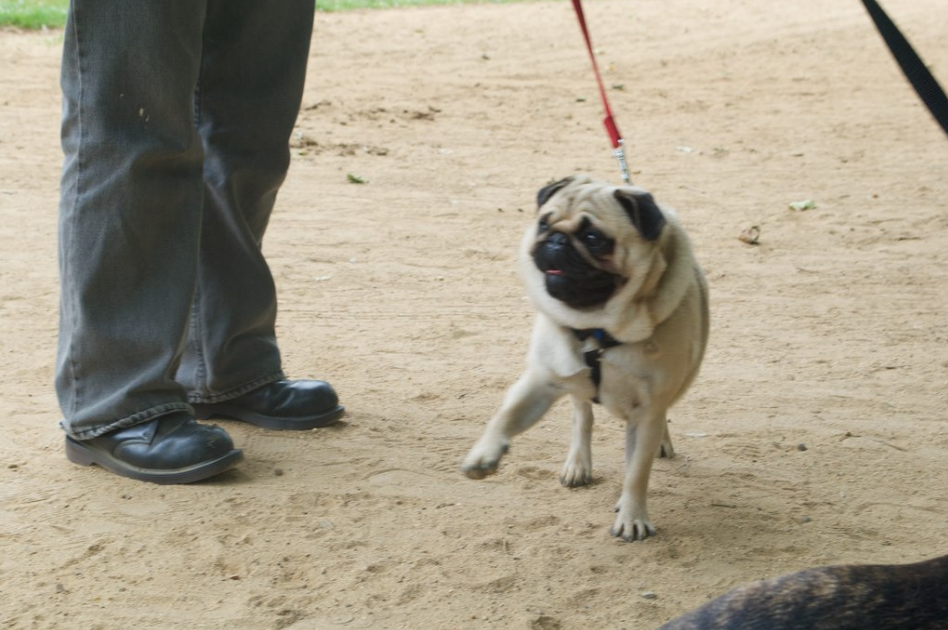
\includegraphics[width=10cm]{../assets/dog-before.png}
   \caption{Naamitoitava kuva}
\end{figure}

\begin{figure}
   \centering
   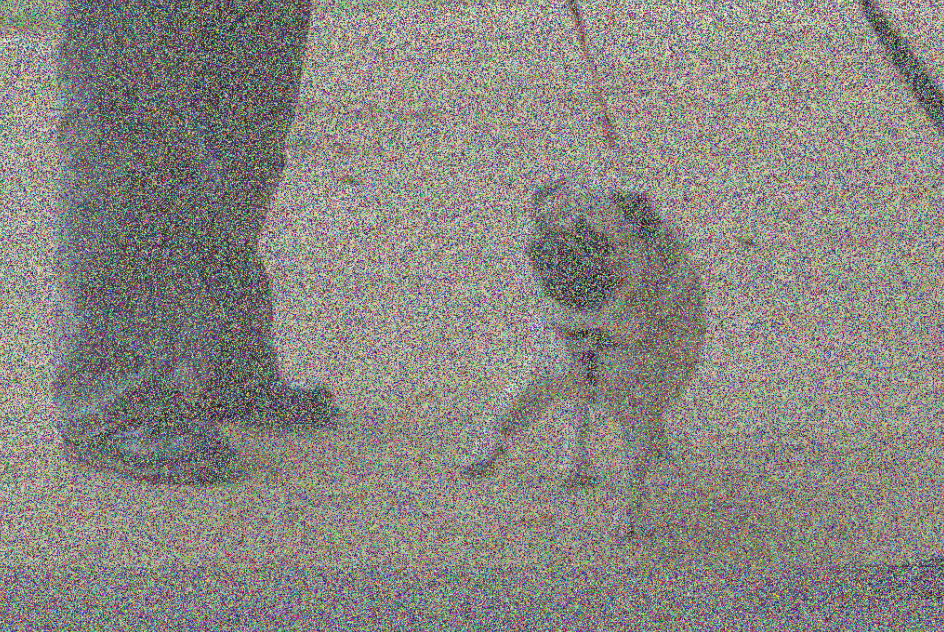
\includegraphics[width=10cm]{../assets/dog-after.png}
   \caption{Ensimmäisessä ja toisessa vaiheessa käsitelty kuva.}
\end{figure}

\section{Puutteet ja haavoittuvuudet}

Sumeita tiivisteitä voidaan yrittää johtaa harhaan eri tavoin. Edellisessä
luvussa käsitellyn haittaohjelman naamioinnin lisäksi menetelmällä, jossa 
harmitonta dataa muokataan tarkoituksellisesti aiheuttamaan osuma jonkin
haitalliseksi todetun sisällön kanssa, voidaan hidastaa haittaohjelmien torjuntaa. 
Haittaohjelmien leviämistä voidaan tehostaa myös kasvattamalla torjuntatyön kuormittavuutta. Kasvanut työmäärä hidastaa haittaohjelmien tunnistamista. Kuormittavuutta voidaan lisätä pyrkimällä aiheuttamaan perättömiä haittaohjelmaepäilyjä. Tällainen
harhautusmahdollisuus on olemassa sumeita tiivisteitä vastaan. \textcite{ermerins} esittää tällaisen uhan erityisesti Ssdeepiä vastaan ja tutkii mahdollisuuksia tulosten vääristelyyn.

\textcite{ermerins} pyrkivät laatimaan menetelmän, jolla olisi mahdollista luoda proseduraalisesti tunnistamattomia kuvia, joiden samankaltaisuus lähdekuvan kanssa olisi suuri. Esitetty menetelmä muokkaa kuvia kahdessa vaiheessa, joista ensimmäisessä luodaan pikseleitä yksitellen muokkaamalla uusi kuva. Tämän kuvan on tarkoitus olla
semanttisesti tunnistamaton, eli ihmisen ei tulisi voida yhdistää niitä
toisiinsa. Edellytyksenä kuitennkin on, että Ssdeep merkitsee osumaksi generoidun kuvan samankaltaiseksi alkuperäisen kanssa. Generoidusta kuvasta luodaan
toisessa vaiheessa nopeasti suuri määrä hieman toisistaan poikkeavia
versioita muuttamalla sattumanvaraisesti valittuja pikseleitä.
Kuvassa 5.1 on tutkimuksessa käytetty alkuperäinen kuva; kuvassa 5.2
on alkuperäisen kuvan käsitelty versio.

Kokeessa havaittiin ssdeep-ohjelmiston kyenneen yhdistämään kaikki generoidut kuvatiedostot alkuperäiseen. Lisäksi generoitujen kuvien huomautetaan olevan ilmeisen
tunnistettavan näköisiä alkkuperäisisen kuvan kanssa. Siten tavoitetta generoida tunnistamattomia kuvatiedostoja ei saavutettu. Lisäksi huomautetaan kehitetyn menetelmän olleen hidas ja sopimaton käytännön sovelluksiin. Tutkimuksessa on esitetty
potentiaalisia optimointikeinoja menetelmän suorituskyvyn kasvattamiseksi.

Datan naamiointia sumeita tiivisteitä vastaan tutkitvat \textcite{oliver14}.
Aiemmin käsitellyn ohjelmien tunnistamisen lisäksi naamiointi suoritettiin
kuva- ja tekstitiedostoille sekä HTML-websivuille käyttäen Ssdeep-, Sdhash-
ja Tlsh-ohjelmistoja. Kuvien naamioinnissa roskapostituksessa
käytettyjä kuvia käännettiin sekä venytettiin, minkä lisäksi
kirjasinkokoa ja -lajia muutettiin. Tekstitiedostoja muutettiin
lisäämällä, poistamalla ja vaihtamalla sanoja, vaihtamalla
rivien paikkaa ja lisäämällä satunnaista dataa. HTML-sivuihin
lisättiin tyhjiä merkkejä sallittuihin kohtiin.

Ssdeepin todetaan suoriutuneen heikoimmin kuvien yhdistämisessä;
Sdhash ja Tlsh suoriutuivat hyvin. Sdhash ei suoriutunut käännettyjen
ja venytettyjen kuvien tunnistamisessa, ja Tlsh tunnisti eniten kuvia.
Tekstitiedostojen muuttaminen aiheutti ongelmia Ssdeepille ja Sdhasille,
Tlsh suoritui paremmin. 500 muokatusta Html-sivuista Ssdeep ja Sdhash
tunnistivat 11 ja 16, ja Tlsh 291. Vertailu osoittaa, että Tlsh suoritui
kaikissa tilanteissa merkittävästi paremmin. Havaitaan, että eri ohjelmistojen
suoriutumisen välillä on merkittäviä eroja, jotka riippuvat syötteen
formaatista. Toiset ohjelmistot reagoivat herkemmin datatyypin
muutokseen tai tarkoitukselliseen harhauttamiseen. Lisäksi
huomautetaan, että erityisesti ohjelmakoodin muuntelu aiheuttaa
em.\ datatyyppejä suuremman haasteen staattiselle
haittaohjelma-analyysille.

\section{Ohjelmistojen erot}

On selvää, että haittaohjelma-analyysissa tutkielmassa käsitelyllyillä
tiivisteohjelmistoilla on mwrkittäviä eroja. Kontekstiriippuvaisten
paloittain määriteltyjen tiivisteiden tunnistuskyky on heikko, ja
Sdhash sekä Mvhash-b vaikuttavat soveltuvan haittaohjelmien tunnistamiseen
paremmin. Erityiseti Ssdeepin ja Sdhashin välillä havaitaan merkittävä
ero tarkkuudessa sekä ohjelmakoodin että muuntyyppisen datan suhteen.

\textcite{martin-perez21} esittävät neljä hyökkäystyyppiä
sumeita tiivisteitä vastaan; samankaltaisuuden vähentäminen
ja simulointi sekä tiivisteiden generoinnin ja vertailun
hankaloittaminen. Hyökkäyksille altistavat tekijät
vaihtelevat, ja suurimmassa osassa ohjelmistoja
esiintyy haavoittuvuuksia. Tutkielmassa
kuvatut ohjelmistot ovat alttiita kaikille
hyökkäystyypeille.

Tietyn ohjelmiston suoriutuminen riippuu suurelta osin tilanteen edellyttämistä
tarpeista ja käsitellyn datan tyypeistä. Sdhashin vahvuuksiin ei kuulu
kokonaisten tiedostojen vertailu, vaan pienempien rakenteiden
havaitseminen \parencite{breitinger12}. Ohjelmistot kärsivät
erilaisista puutteista toteutuksessa.


\chapter{Yhteenveto\label{summary}}
Samankaltaisuuden
tunnistamiseen on ollut tarvetta monessa paikassa,
ja aiemmat ratkaisut eivät ole tähän kyenneet. Erityisesti
tarvetta on haittaohjelmien tunnistamisessa, jossa on perinteisesti
käytetty kryptografisia tiivisteitä. Ongelmaa lähestyvät
sumeat tiivisteet mahdollistavat samankaltaisten haittaohjelmien
tunnistamisen.

Sumea tiivistys on uudehko tekniikka, mutta sumean tiivistyksen
ohjelmistoja on kehitetty laajasti. Eri ohjelmistot lähestyvät
samankaltaisuuden tunnistamista poikkeavin tavoin, mikä on tehnyt
vertailun ja luokittelun haastavaksi. Ohjelmistoista käsiteltiin
tunnetuimpiin kuuluvat ominaisuusjonoja tiivistäväþ Ssdeep ja Sdhash
sekä hieman uudempi Mvhash-b, joka keskittyy tavujonoihin.

Kaikki kolme käsiteltyä sumean tiivistyksen ohjelmistoa poikkeavat
toteutustavaltaan radikaalisti toisistaan. Poikkeavat esitystavat
samankaltaisuudelle vaikeuttavat ohjelmiston valintaa. Toiset
ovat päällekkäisiä, toiset taas aivan erilaisia. Ohjelmistojen
soveltuvuutta haittaohjelma-analyysin tarpeisiin pohdittiin
perinteisten haittaohjelmien tunnistamiskeinojen ja torjuntatyön
edellytysten pohjalta; tästä edettiin analysoimaan menetelmiä, joilla
haittaohjelmien tekijät voivat harhauttaa sumein tiivistein
tehtävää torjuntatyötä.

Lopuksi käsiteltiin rajoitteita, joita sumeat tiivisteet
tuovat mukanaan. Yleiseten rajoitteiden lisäksi
käesiteltiin Ssdeepin, Sdhashin ja Mvhash-b:n
toteutusten puutteita ja hyökkäysalttiutta, sekä
verrattiin toteutusten eroavaisuuksien ilmenemistä
käytännössä. Läpi käytiin myös sumeiden tiivisteiden
haavoittuvuuksia sekä näitä hyödyntäviä potentiaalisia
hyökkäyksiä.


%%%%%%%%%%%%%%%%%%%%%%%%%%%%%%%%%%%%%%%%%%%%%%%%%%%%%%%%%
%\cleardoublepage                          %fixes the position of bibliography in bookmarks
%\phantomsection
\addcontentsline{toc}{chapter}{\bibname}  % This lines adds the bibliography to the ToC
\printbibliography

%%%%%%%%%%%%%%%%%%%%%%%%%%%%%%%%%%%%%%%%%%%%%%%%%%%%%%%%%
\backmatter

\end{document}
